%% Full length research paper template
%% Created by Simon Hengchen and Nilo Pedrazzini for the Journal of Open Humanities Data (https://openhumanitiesdata.metajnl.com)

\documentclass{article}
\usepackage[english]{babel}
\usepackage[utf8]{inputenc}
\usepackage{johd}
\usepackage{hyperref}

\title{National Hockey League Network Analysis}

\author{Emmett Collings$^{a}$$^$, Banafsheh Khazali$^{b}$$^$ \\
        \small $^{a}$CPSC 572, UCID: 30076370 \\
        \small $^{b}$CPSC 672, UCID: 30163247 \\}

\date{} %leave blank

\begin{document}

\maketitle
\begin{abstract} 
\noindent The National Hockey League (NHL) is considered to be the top-ranked professional ice hockey league in the world. Sports leagues are hyper-competitive and it is consistently shown that more successful teams competitively have immediate financial success as well. The current state of hockey analytics is largely focused on individual contributions. The goal of this project is to expand beyond individual contributions and attempt to formally quantify the notion that players can have significant impacts on the effectiveness of their teammates. For this study, we sampled the statistics of NHL players for the past 10 years. We found that players who are relatively better than their teammates tend to have a larger impact on their teammates while increasingly while increasingly fringe players have lesser to deleterious effects. We can also infer that effective combinations of players often arise
when the players have some sort of statistical similarity and they are more effective when they play with similar players.
 \end{abstract}



% \noindent\authorroles{For determining author roles, please use following taxonomy: \url{https://credit.niso.org/}. Please list the roles for each author.} 

\section{Research questions}
We aim to investigate the following research questions in this paper:
\begin{enumerate}
    \item Can we identify what NHL players improve their teammates the most, and can we identify any trends or play style details about these players?
    \item Can we identify groups of players that specifically improve each other more than an average player?
    \item Can we identify certain play styles or characteristics that tend to disproportionately impact other play styles or characteristics?
    \item Can we generate any predictions on players that may improve players that they have not played with yet?
\end{enumerate}


\section{Introduction}
National Hockey League (NHL) is one of the four major professional sports leagues in the United States and Canada\href{https://en.wikipedia.org/wiki/Season_structure_of_the_NHL}{(Wikipedia)}. In team sports, like hockey, there is immense pressure to perform at a high level. To help perform at a high level, analytics have infiltrated the sports world. Analytics problems in sports are vast and include important problems such as player evaluation and scouting, player development, modification of tactics, and working on team combinations to improve the game \cite{foster2021playing}. These problems are becoming increasingly complex and require knowledge to capture the current state of the rapidly changing world of hockey analytics.\par
The goal of any professional hockey team is to win, and assembling a good team is a component of winning. In makings of a good team in the NHL, we must consider  many factors such as team synergy, team depth, and salary cap constraints, but there is no doubt that the evaluation of individual talent is crucial in building a good team \cite{guan2022game}. Although coaches have a strong sense of the contributions of players, sometimes there may be subtleties about player contributions that remain undetected. Therefore, objective measures of player evaluation form part of the evaluation process.\par
There are lots of hockey analytics problems whose solutions are straightforward \cite{vollman2016hockey}. For example, a team may want to know the proportion of face-offs that are won by a particular player. As useful as this information may be to teams, we do not consider straightforward research investigations in this paper. Despite this, we see how we can use some statistics like ice Corsi percentage and off-Corsi difference to investigate team success, players\textsc{\char13}  impact on other teammates, and how to pair up players to yield better results. \par
In Section 3, we describe data that are available for hockey players\textsc{\char13} analytics and details on how we can construct a network based on NHL players\textsc{\char13} information. In Section 4, basic statistics and their usage to answer the main questions are explained. We provide network visualization in section 5, followed by results in section 6 where we can see what players frequently had large impacts on the quality of their teammates\textsc{\char13} play and what an effective team combination is. The purpose of section 7 is to compare our network with two null models. We conclude with a short discussion in Section 8. More details about the methods and the source code for this study can be found in sections 9 and 10, respectively.



\section{Dataset description}
To observe community structures and answer our research questions, we needed to collect a large amount of hockey game data. Since the 1995–96 season, each team in the NHL plays 82 regular season games \href{https://en.wikipedia.org/wiki/Season_structure_of_the_NHL}{(Wikipedia)} and we wanted to collect data from a broad time range so we could study the effectiveness of players on each other. Given these requirements, a subset of NHL games information between 2011 to 2021 proved a perfect sampling set. The dataset is publicly available on moneypuck \href{https://moneypuck.com/data.htm}{(Moneypuck.com)}. In total, we downloaded 20 CSV files containing single season data on skaters and Line/pairing information. 

\subsection{Network construction}
The nodes in our directed-weighted network are NHL players. Two players are connected by an edge if they have been deployed together for more than 600 minutes over the past 10 years. The edge weight is the difference in a player's Corsi percentage when deployed with and without the other player. Thus the weights can be positive or negative. 
If player X has an effect on player Y, then the edge (X,Y) has the magnitude of this effect as its weight.
Furthermore, NHL players are most often deployed in discrete units of defensemen pairs and forward lines. 
Players very rarely play as both defencemen and as forwards over their careers, so we divided our players into two categories of defencemen and forwards to illustrate the mostly separate populations.
The direction of the edges is based on the effect a player has on another.

\section{Network statistics}
After creating the two networks, we computed and compared their basic statistics, shown in Table~\ref{tab1}. The average path length for the network is more than 3 which is expected since both networks exhibit small-world properties displayed by their degree distributions in \textbf{Fig.~\ref{fig1}} and \textbf{Fig.~\ref{fig2}}. 

\begin{table}[H]
\centering % Label your table accordingly

\begin{tabular}{ccc}
\hline
Measures & Defencemen Network & Forwards Network  \\
\hline
Number of nodes &  416 & 802  \\
Number of edges & 4206 & 7114\\
Number of connected components & 2 &2 \\
Number of communities & 14 & 20\\
Avg. degree & 10.11 &  8.87\\
Avg. path length & 3.35 & 3.46 \\
Clustering coefficient & 0.497 & 0.613 \\
\hline
\end{tabular}
\caption{Basic statistics of our networks}\label{tab1}
\end{table}

\begin{figure}[H]
\centering
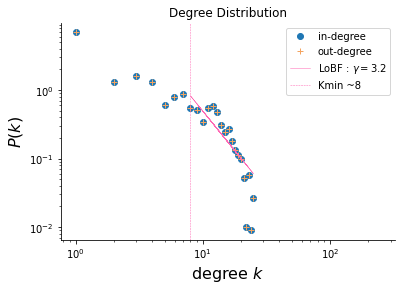
\includegraphics{images/powerlaw.png}
\caption{\label{fig1}Log-log plot of degree distribution for defencemen network and its fit. The network has a $\gamma > 3$ which means the network is in the small world regime.}
\end{figure}

\begin{figure}[H]
\centering
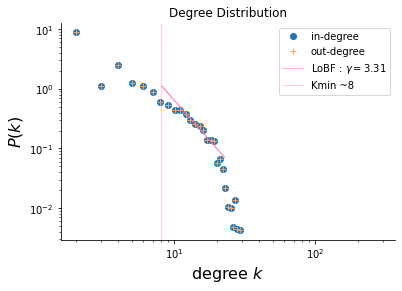
\includegraphics{images/1.png}
\caption{\label{fig2}Log-log plot of degree distribution for forwards network and its fit. The network has a $\gamma > 3$ which means the network is in the small world regime.}
\end{figure}

The network measures we choose to compute for our networks are weighted out-degree,  correlation coefficient, clustering coefficient, modularity, and the average shortest path length. The average weighted out-degree and correlation coefficient can be used to identify players\'s actual effects on individual teammates. The modularity, clustering coefficient, and average shortest path length  were used to compare with our null models. 


\section{Network Visualization}
See the appendix for full size images of our visualizations.
Full visualizations of our defense and forwards networks can be found at \ref{vis1} and \ref{vis2} respectively.
For these visualizations the size of the nodes scale with total out-degree, indicating which players have had the greatest collective positive impact on their teammates.
The colors correspond to communities generated via Gephi's modular community detection algorithm.
In a league with 32 teams, the relatively low number of communities generated in either the forwards or defense graph is indicative of relatively high turnover over our time period.
This is generally promising as there will likely be less correlation between teams and the type of players that players play well with.

We also have included visualizations of the positive edge only defense and forward networks at \ref{vis3}, and \ref{vis4}.
These follow the same scheme as the full network visualizations, except that the communities generated are those that we analyzed in section \hyperref[sec:community]{6.2}.
The increased number of communities in these subgraphs relative to the full networks is a promising indication that we may find some interesting results.
Higher levels of differentiation between communities of players that simply played with each other vs players that played well with each other indicates that there may be some trends that we can identify and make inferences about.

\section{Results}
\subsection{Influence Correlations}
Our first research question was to identify what players frequently had large impacts on the quality of their teammates' play.
In our network, weighted out-degree is analogous to the total influence a player had on all their teammates.
There are several factors that suggest that this metric alone is not fully representative of a player's influence.
Players with longer careers or who have been traded frequently often have far larger sets of players that they have played with.
This can have the effect of increasing their total influence while their actual effects on individual teammates may be lesser than others.
To account for this, we decided to rank players instead by their average outgoing link weight.
Apart from just ranking players by this metric, we also sought to characterize players that tended to have larger influencing effects.
To assess this, we calculated the correlation between various individual statistics and average outgoing influence for the player base as a whole.
We used the Spearman correlation coefficient as it is better suited to our discrete data, and visually inspected charts of our data to detect any potentially non-monotonic relationships, of which there appeared to be none.
Our results are given in table \ref{correlation}.

\begin{table}[H]
    \centering
    \begin{tabular}{ccc}
    \hline
        Statistic & Forwards & Defense \\ \hline
        On Ice Corsi Percentage & 0.6033 & 0.7249 \\ 
        Off Ice Corsi Percentage & 0.1302& 0.1554 \\ 
        On Off Corsi Difference & 0.5310& 0.6541 \\ 
        On Ice Goals For per 60 & 0.2805& 0.2381 \\ 
        On Ice Goals Against per 60 & -0.0621&-0.1784 \\
        DZone Giveaways per 60 & 0.0491& 0.0101 \\ 
        Giveaways per 60 & 0.1679& 0.0500 \\ 
        Hits per 60 & -0.1291& -0.2075 \\ 
        Takeaways per 60 & 0.2833& 0.2625 \\ 
        Shots Blocked per 60 & -0.2140& -0.2816 \\ 
        Primary Assists per 60 & 0.2157& 0.2952 \\ 
        Secondary Assists per 60 & 0.2542& 0.1977 \\ 
        Goals per 60 & 0.2166& 0.1989 \\ 
        Points per 60 & 0.2843& 0.2901 \\ 
        \hline
    \end{tabular}
    \caption{Spearman correlation coefficients for individual statistics vs average outgoing influence. For an explanation of the statistics listed see the data dictionary in our Github repo.}
    \label{correlation}
\end{table}
We can draw several conclusions about players that then to improve the play of their teammates from this.
The strongest correlations we have are with on ice corsi percentage and on off corsi difference.
Corsi percentage is generally considered an effective single metric predictor of team success, indicating the biggest influence on a players' impact on teammates is their overall quality (perhaps unsurprisingly).
On off corsi difference is the difference in the teams corsi percentage when a player is actively on the ice vs when they are on the bench.
Higher corsi differences indicate that a player is significantly better than the rest of their team or disproportionately contribute to the teams success.
The high correlation here is also somewhat unsurprising; players relatively much better than their teammates tend to have a larger impact on those teammates.
The relatively weak correlation for our other tested statistics may indicate that a variety of approaches may be effective for increasing teammate impact.

It's important to mention that we cannot claim any causal relationship between any of these statistics.
Some confounding factors can arise that could explain some phenomena that initially seem paradoxical.
For example, giveaways are invariably a bad play that shuts down any isolated play and gives the opposing team a chance to have possession.
However, for forwards they are weakly positively correlated with teammate impact.
In this case, it's likely that higher amounts of giveaways correspond with higher possession figures in general, and thus allowing players more opportunity to generate more offense on a macroscopic level.

\subsection{Community Analysis}
\label{sec:community}
Our second and third research questions concerned the characterization of players that would tend to specifically benefit each other, as opposed to finding general information about positive teammate impact players.
To accomplish this, we focused our efforts on beneficial relationships i.e. edges with a positive weight.
We removed all negative and zero-weighted edges from our complete graph, and ran a community detection algorithm on the resulting subgraph.
By identifying and characterizing communities of players that tend to strongly connect with each other we can analyze trends within these communities that differ from less positive partnerships.

Our choice of algorithm was Clauset-Newman-Moore greedy modularity maximization to find the partition with the largest modularity.
Choosing a partition method based on modularity would yield groupings of players with dense positive connections amongst themselves, hopefully giving groupings of players that perform well with each other even if they have not yet directly interacted.
The rationale behind choosing this specific algorithm was mostly due to outputs that were more interesting.
Alternatives such as the Louvain algorithm tended to partition our graphs into high numbers of very small communities, which correspondingly had less statistical power when compared to the entire player base.

Using the networkx function \texttt{greedy\_modularity\_communities()} we ended up partitioning our forwards graph into 20 communities and the defensemen into 23.
We then investigated characteristics of these communities by comparing the community mean of the individual player statistics with the mean of the entire player base, using 1 sample t tests to determine with 95\% confidence if they were different.
Our results determined that most communities in one stat or another are significant outliers from the distribution of the population.
For any particular statistic on average 45\% of communities would have a different mean from the population.
This is indicated that at least in some respects players with highly similar statistics tended to synergize more effectively with each other instead of players with markedly different playstyles.
If effective combinations were based off of complementary playstyles we would expect most communities to exhibit trends in line with the population.

To further investigate the phenomenon of players being more effective with similar players, we performed the same analysis except on the subgraph containing only negatively weighted edges.
With the exception of team-based stats (such as corsi percentage, on ice goals for, etc.) there were far less communities that exhibited the same biased distributions.
While the proportion of communites per stat that had differing means from the population was 30\% (still lower than the positive network), this was characteristically due to a smaller amount of communities with a wider variety of varying stats.
In other words, a relatively larger portion of negative communities displayed no meaningful statistical differences from the population.
For team based stats we did find some interesting exceptions.
Many negatively influencing communities actually had significantly higher general contribution stats, most notably corsi percentage.
This combined with the lack of differentiation in individual stats may be indicative that haphazardly pairing up similarly elite players but with vastly different play styles is ineffective at yielding better teammate impacts.

Overall from this community analysis we can infer that effective combinations of players often arise when the players have some sort of statistical similarity.

\section{Comparison to null models}
The networks in this project are weighted and directed. The null models we used are the a. random ER network and b.degree-preserving configuration model. 
a. To compare our models with a random ER model, we first considered a network with the same number of nodes based on the node sizes of our two networks. Then directed links were randomly assigned to the nodes. Since our network is weighted, edge weights in the same range as our network were assigned to the links. 
b. For the degree-preserving model we performed two randomization stages: first edges were randomized via randomly swapping links while keeping the degree distribution of the original networks. At this stage, we made sure that the in-degree and the out-degree of each node are not changed. After the link swapping the resulting network is an unweighted network. Because link weights affect the community detection algorithm, we then randomly assigned edge weights to each link. The ranges of the randomly generated weights correspond to the actual network’s minimum and maximum edge weights. \par
We generated an ensemble of 1000 null models for each graphs. The modularity value is given by the Clauset-Newman-Moore greedy modularity maximization  algorithm and an average was calculated. The number of connected components, clustering coefficient, and average shortest path were calculated and averaged over the ensembles in Python. The results are shown in Table~\ref{tab2} and Table~\ref{tab3} \par
\begin{table}[H]
\centering % Label your table accordingly

\begin{tabular}{cccc}
\hline
Measure & Real data & DP($\pm \sigma$) & ER($\pm \sigma$)\\
\hline
Connected Components &  2 & 1 & 1\\
Clustering Coefficient & 0.497 & 0.210 $(\pm0.003)$ & 
0. 0487 $(\pm0.007)$\\
Modularity & 0.627 & 0.485$(\pm0.002)$ & 0.275$(\pm0.002)$\\
Average Path Length & 3.513 & 3.020 $(\pm0.041)$ & 2.31 $(\pm0.08)$ \\
\hline
\end{tabular}
\caption{Comparison of modularity, connected components, clustering, and average path length of the defencemen network with its null models, where $\sigma$ is the standard deviation for each measure.}\label{tab2}
\end{table}
The modularity and clustering coefficient of our forward and defencemen network were higher than null models, including standard deviation. We calculated the number of connected components and considered their mode of them, which was 1, indicating that the null models became a single giant connected component, while our network had 2 components including one giant component. These observations confirm that the grouping of our nodes is not random, and neither are the edge weights of our network. The average path length stayed consistent between null models and our networks. This is expected since the degree distribution of both networks are not changed. $ {\gamma}$ and average path length for both networks are greater than 3 which is the signature of the small-world property characterizing random networks. 
\begin{table}[H]
\centering % Label your table accordingly

\begin{tabular}{cccc}
\hline
Measure & Real data & DP($\pm \sigma$) & ER($\pm \sigma$)\\
\hline
Connected Components &  2 & 1 & 1\\
Clustering Coefficient & 0.613 & 0.317 $(\pm0.004)$ & 0.11$(\pm0.007)$\\
Modularity & 0.743 & 0.381$(\pm0.002)$ & 0.199$(\pm0.007)$\\
Average Path Length & 3.513 & 3.3 $(\pm0.033)$ & 4.25 $(\pm0.08)$ \\
\hline
\end{tabular}
\caption{Comparison of modularity, connected components, clustering, and average path length of the forward network with its null models, where $\sigma$ is the standard deviation for each measure.}\label{tab3}
\end{table}


\section{Discussion}
The current body of hockey statistics largely focuses on contributions made on an individual level.
Existing statistical work has been done comparatively sparingly on the effects that players have on categories of teammates.
Currently, with or without you stats (aka WOWY) track this difference between when a player is deployed with or without a specific player, but do not expand any further beyond individual instances.
This kind of analysis forms the basis of our calculated edge weights.
However, the expansion of this kind of analysis beyond specific player combinations and into macro trends via networks has not seen much development as of yet.
This line of analytics is thus relatively unexplored and a potentially lucrative direction to focus research efforts on.

Our first research question pertained to general trends that we could identify among players that had high impacts on their teammates.
This would be a generally interesting investigation for coaches and hockey analysts because if we could identify certain aspects that were unusually correlated we could perhaps then identify strategies or play styles that were more effective than others.
Overall, we didn't find anything specific that highly correlated with positive impacts.
The overall calibre of a player was the greatest indicator that they would improve the gameplay of their teammates.
The correlations we found among individual stats and average outgoing influence are actually quite similar to correlations with general offensive stats.
For example, hits per 60 is negatively correlated with average influence as well as goals for per 60.

Our second third and fourth research questions aimed to analyze what makes effective pairings of players effective.
While we gained some insight that effective pairings often consist of players with similar strengths, a weakness of our approach to this was the inability to conclusively rule out complementary but differing playstyles.
Negatively impactful communities tended to not display concentrations of specific playstyles, instead involving a variety of players of differing effectiveness.
The positively impactful communities displayed some communities with highly skewed distributions of certain individual statistics, but there were also several instances of distributions similar to that of the negative communities.
A possible explanation for this behaviour is that amongst these positive relationships are players with complementary playstyles that are emphasized by different statistical profiles but nevertheless efficient at helping their team.
To effectively analyze this we would = have to investigate more carefully the relationship and potential correlation between the magnitude of edges between nodes that large differences in their individual statistics.

Another direction to take to build on this network is to incorporate more third party metrics that were not made available in our base dataset.
Many modern advanced analytics are computed with models that account for a greater amount of context than the basic statistics we used, such as strength of competition, offensive/defensive utilization, and coaching style effects among others.



\section{Methods}
\subsection{Degree Distribution}
For finding a power law fit for our degree distribution we need some more steps. Early on in our analysis, we used a python library called Scipy and used its function curve fit to find a power law fit for our degree distribution. But Scipy curve fit fails, as it accommodates all of the nodes and fits one line for all data. 
Reading Advanced Topic Section 3 from the Network Science Book helped us proceed. A link to a project by Aaron Clauset \cite{clauset2009power} provided a code base to fit a power law to real data. The algorithm attempts to fit a power law to every partition of the degree distribution based on a specific $K_{min}$. It calculates the log-likelihood of the data $K \geq K_{min}$ fitting the power law for each partition. It outputs the $K_{min}$ and $\gamma$ values for this best fit. 
For our networks, it found $K_{min} = 7.97$  and $\gamma = 3.2$ for defencemen network, and $K_{min} = 7.97$  and $\gamma = 3.31$ for forwards network.  With these two $K_{min}$ almost 65\% of the networks were included in the fit. This selected $K_{min}$ also visually seemed to indicate where our degree distribution looked like it could be fitted with a power law. 
To calculate the constant C for the power law fit, we referred to equation (4.12) from the Network Science textbook \cite{Barabasi} which is reflected in Clauset paper on fitting power laws to empirical data. For defencemen network C = 42, while for forwards C = 32.
\begin{equation}
p(k) = Ck^\gamma
\end{equation}

\begin{table}[H]
\centering % Label your table accordingly

\begin{tabular}{ccc}
\hline
Measure & Defencemen Network & Forwards Network\\
\hline
$\gamma$ &  3.2 & 3.3\\
$k_{min}$ & 7.97 & 7.98\\
C & 32 & 42\\
\hline
\end{tabular}
\caption{Comparison of modularity, connected components, clustering, and average path length of the forward network with its null models, where $\sigma$ is the standard deviation for each measure.}\label{tab3}
\end{table}


\subsection{Network disassortativity}
Hubs in networks are expected to link to each other but in some networks they do and in others they don't. According to the calculations that we had in our networks, hubs do not have the tendency to link to other hubs which shows the disassortativity in both of our networks. It fits our findings about our networks that the most important nodes link with less important nodes to make them better. The disassortativity of the whole network is shown in \textbf{Fig.~\ref{fig3}}.
\begin{figure}[H]
\centering
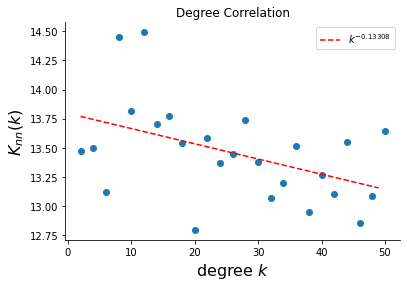
\includegraphics{images/disfor.png}
\caption{\label{fig3}The degree correlation for the whole network. The negative slope shows that the network is disassortative. }
\end{figure}

\subsection{Spearman Correlation Coefficient}
After calculating our total outgoing influence and average outgoing influence, we wanted to see if we could find any trends in a player's individual statistics.
To accomplish this, we copied their average outgoing influence back into the players dataframe and computed the correlation matrix (available on our GitHub repo in the data section).
The coefficient we used was the Spearman method, appropriate for discrete data and capable of finding monotonic relationships (not necessarily linear) between different data distributions.
We additionally inspected scatterplots of our data in question to evaluate whether any data had relationships that would not be represented by the Spearman coefficient, such as quadriatic.
The implementation used was the Spearman rank correlation python implementation in the numpy library.

\subsection{Community Characterization}
To determine whether our observed statiscal means within our communities were different than those of the population we first calculated the population mean.
We then input our community statistics and the population mean into a 1 sample t test.
The implementation used was \texttt{scipy.stat.ttest\_1samp()}.
The 1 sample t test essentially takes into account the sample size and standard error to compare a sample with a fixed mean.
We used a confidence interval of 95\% as our threshold of being significantly different from the population.
In our code, this equates to a p-value of less than 0.05.


\section{Code}
Our initial data, processed data, code, and visualizations are available online on \hyperlink{https://github.com/emmettcollings/nhl-linemate-network}{Github}.
A short description of what each module used to create this paper are provided in table \ref{code}.

\begin{table}[H]
\centering
\begin{tabular}{|l|p{6cm}|}
\hline
File & Description \\
\hline
aggregate-forwards.py             & Processes forward data season by season, aggregating statistics and transforming into rate statistics as required. \\ \hline
aggregate-lines.py                & Aggregates line data season by season, combining lines that appear across multiple teams and season as required. \\ \hline
create-forwards-corsi-edgelist.py & Creates edges between players by aggregating instances of them playing together. \\ \hline
forwards-overall.ipynb            & Used for network analysis and visualization of the overall forwards network. \\ \hline
forwards-positive.ipynb           & Used for network analysis and visualization of the positive only forwards network. \\ \hline
\end{tabular}
\caption{Python files used for the NHL network analysis}
\label{code}
\end{table}

Analogous files exist for creating the defense network.
All code written is original.
Networkx implementations were used for all network analysis techniques.


\newpage
\section{Appendix}
\begin{figure}[H]
\centering
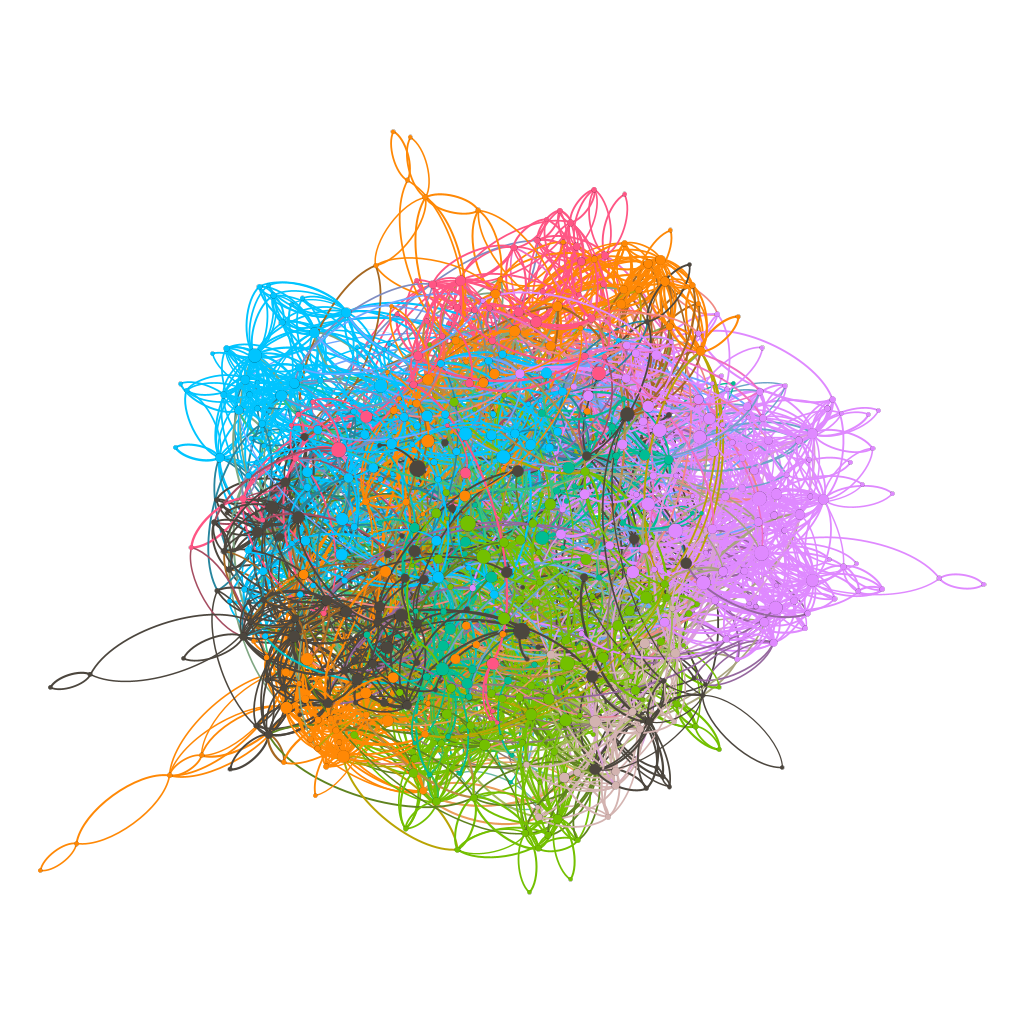
\includegraphics[scale=0.45]{images/defense.png}
\caption{Full Defense Network Visualization}
\label{vis1}
\end{figure}

\begin{figure}[H]
\centering
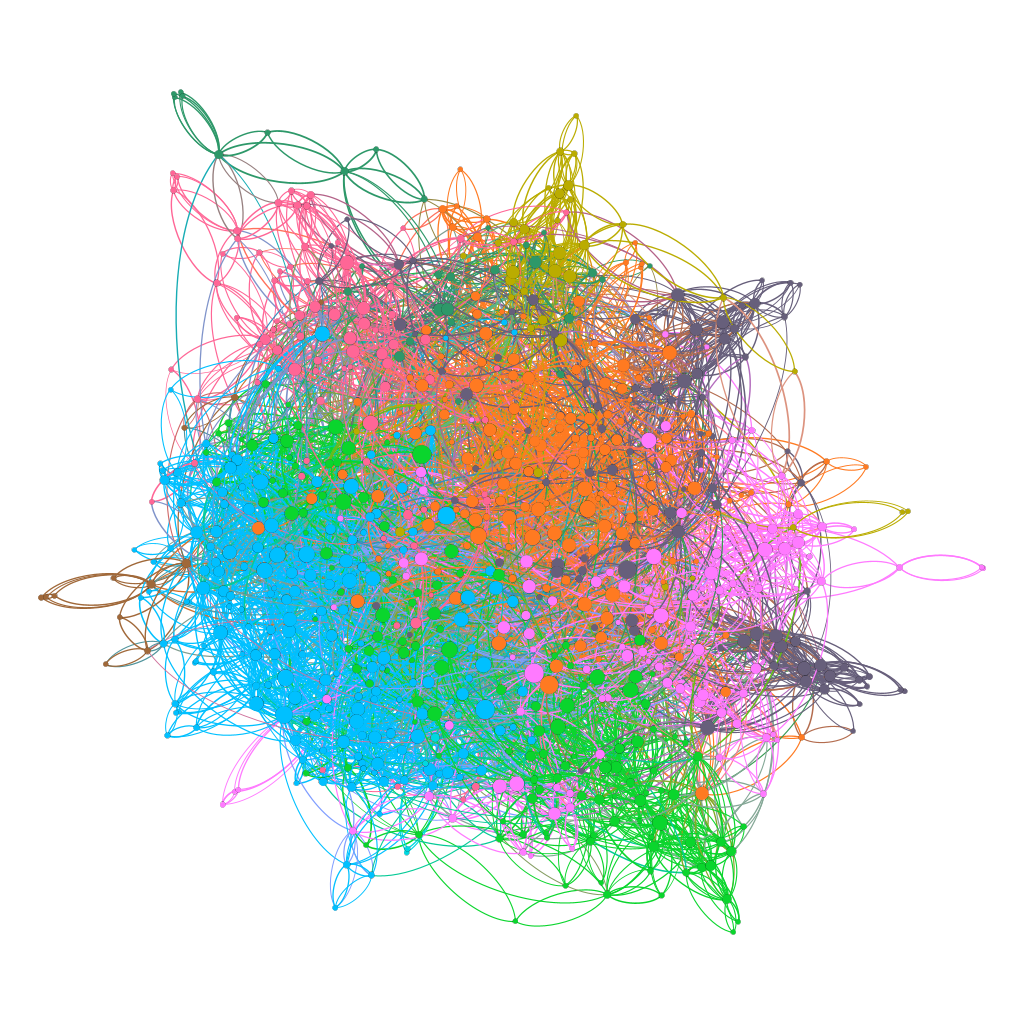
\includegraphics[scale=0.45]{images/forwards.png}
\caption{Full Forward Network Visualization}
\label{vis2}
\end{figure}

\begin{figure}[H]
\centering
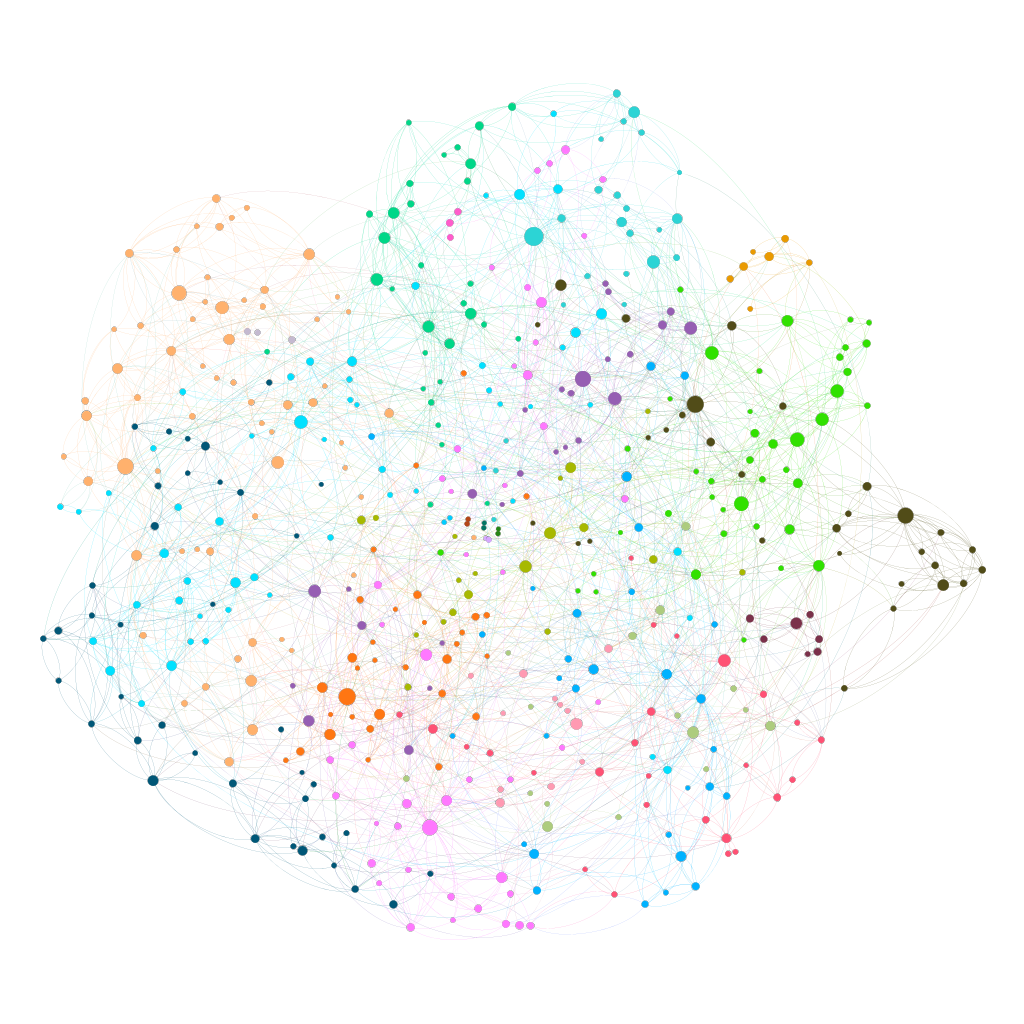
\includegraphics[scale=0.45]{images/defense-positive.png}
\caption{Positive Only Defense Network Visualization}
\label{vis3}
\end{figure}

\begin{figure}[H]
\centering
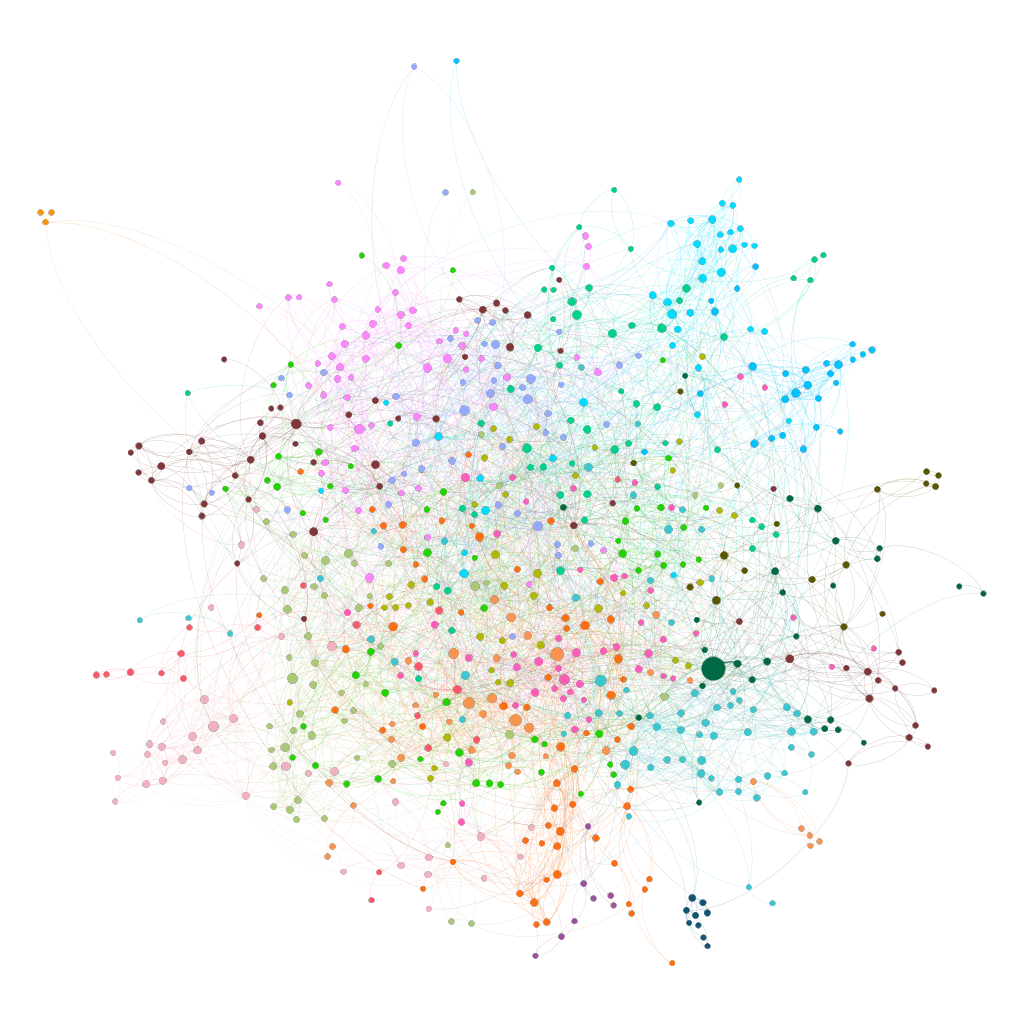
\includegraphics[scale=0.45]{images/forwards-positive.png}
\caption{Positive Only Forward Network Visualization}
\label{vis4}
\end{figure}


% This journal uses a style based on the APA system (see \href{https://openhumanitiesdata.metajnl.com/about/submissions/#References}{here}). \\
% The following are some basic citation commands in \LaTeX: \\

% \noindent
% \verb|\citet| $\rightarrow$ \citet{jenset&mcgil}\\
% \verb|\citet| $\rightarrow$ \citet{australiashealth}\\
% \verb|\citet| $\rightarrow$ \citet{shree-a}\\
% \verb|\citep| $\rightarrow$ \citep{fabricius-hansen2012b}\\
% \verb|\citealp| $\rightarrow$ (\citealp{eckhoff2018a})\\
% \verb|\citealp| $\rightarrow$ (\citealp{eckhoff2018a}; \citealp{fabricius-hansen2012b}; \citealp{shree-a})\\

% \subsubsection{Other simple functions}
% To add bullet points:

% \begin{itemize}
%     \item Some point
%     \item Another point
% \end{itemize}

% \noindent Or numbered points:

% \begin{itemize}
%     \item[1.] Some numbered point
%     \item[2.] Another numbered point
% \end{itemize}

% \noindent This is an example of footnote\footnote{This is a footnote}. \\



% \section{Dataset description}
% Here you can provide, if applicable, information about the dataset(s) whose creation, collection, management, access, processing or analysis have been discussed in this paper, following this schema:
% \paragraph{Object name} Typically the name of the file or file set in the repository.
% \paragraph{Format names and versions} E.g., ASCII, CSV, Autocad, EPS, JPEG, Excel, SQL, etc.
% \paragraph{Creation dates} The start and end dates of when the data was created (YYYY-MM-DD).
% \paragraph{Dataset creators} Please list anyone who helped to create the dataset (who may or may not be an author of the data paper), including their roles (using and affiliations).
% \paragraph{Language} Languages used in the dataset (i.e., for variable names etc.).
% \paragraph{License} The open license under which the data has been deposited (e.g., CC0). 
% \paragraph{Repository name} The name of the repository to which the data is uploaded. E.g., Figshare, Dataverse, etc. 
% \paragraph{Publication date} If already known, the date in which the dataset was published in the repository (YYYY-MM-DD).


% \section*{Acknowledgements}




\newpage
\bibliographystyle{johd}
\bibliography{bib}
https://github.com/emmettcollings/nhl-linemate-network



\end{document}